\documentclass[14pt]{beamer}
\title{WEB :: HTML}
\author[TS]{TalentSprint}
\institute[L\&D]{Licensed To Skill}
\usefonttheme{serif}
\usecolortheme{orchid}
\usepackage{bookman}
\usepackage{hyperref}
\usepackage[T1]{fontenc}
\usepackage{graphicx}
\usepackage{listings}
\graphicspath{{./../Images/}}
\usepackage{tikz}
\usepackage{soul}
\usepackage{color}
\beamertemplateballitem
\usebackgroundtemplate{
\includegraphics[width=\paperwidth]{TS-XP-Logo.jpg}}
\lstset{language=html, numbers=left, numbers=none, basicstyle=\footnotesize, numberstyle=\tiny,  numbersep=10pt, showstringspaces=false, breaklines=true,keepspaces=true, columns=flexible}
\begin{document}

\begin{frame}
  \titlepage
\end{frame}

\begin{frame}{HTML Basics}
The content in this presentation is aimed at teaching  learners to:
  \begin{itemize}
  \item Create hyperlinks that navigate to different WebPages
  \item Display data in a structured format using HTML tables
  \end{itemize}
\end{frame}

\begin{frame}{Hyper Links}
Use anchor tag <a> to create a link.

\lstinline!<a href="url">Text to be displayed</a>!
\begin{itemize}
\item The href attribute is used to indicate the page we are linking to.
\item The target attribute defines where the linked document will be opened. 
\item \_blank, \_parent, \_self, \_top, frame\_name can be the values of the target attribute.

      \lstinline!<a href = ``url'' target = ``_blank''>Text to be displayed</a>!
\end{itemize}
\end{frame}

\begin{frame}{Hyper Links}
\lstinline!<a href = ``www.google.com'' target = ``\_blank'' name = ``glink''> Google Pages </a>!
\end{frame}

\begin{frame}{Tables}
 \begin{figure}[H]
  \centering
  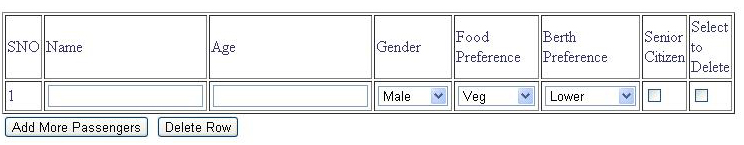
\includegraphics[scale=.4]{s02-tables.png}
 \end{figure}
\begin{itemize}
 \item An HTML table is an element comprised of rows and columns
 \item Tables are container elements, and their sole purpose is to house other HTML elements and arrange them in a tabular fashion -- row by row, column by column
\end{itemize}
\end{frame}

\begin{frame}{Tables}
 \begin{description}
  \item [<table>] tag defines the table
  \item [<tr>] tag divides the table into rows
  \item [<td>] tag divides the rows into cells
 \end{description}
 A data cell can contain text, images, lists, paragraphs, forms, horizontal rules, tables, etc.
\end{frame}

\begin{frame}[fragile]{Tables}
 A Simple Table
 
 \begin{minipage}{6cm}
  \begin{lstlisting}
<table>
    <tr>
        <td>row  1,  cell  1</td>
        <td>row  1,  cell  2</td>
    </tr>
    <tr>
        <td>row  2,  cell  1</td>
        <td>row  2,  cell  2</td>
    </tr>
</table>

\end{lstlisting}
\end{minipage}
\quad
\begin{minipage}{3cm}
 \begin{figure}[H]
  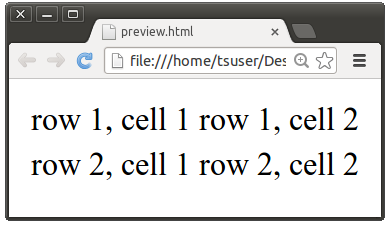
\includegraphics[scale=.3]{s02-tables-ex.png}
 \end{figure}
\end{minipage}
\end{frame}

\begin{frame}[fragile]{Tables}
 Table with Border Attribute
 
\vspace{1pc}
\begin{minipage}{6cm}
\begin{lstlisting}
<table  border = ``1''>
    <tr>
        <td>Row  1,  cell  1</td>
        <td>Row  1,  cell  2</td>
    </tr>
</table>
\end{lstlisting}
\end{minipage}
\quad
\begin{minipage}{3cm}
 \begin{figure}[H]
  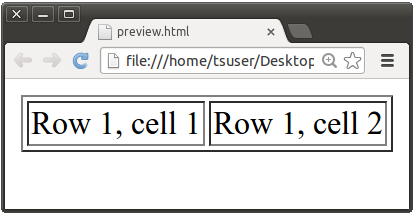
\includegraphics[scale=.3]{s02-tables-border.png}
 \end{figure}
\end{minipage}
\end{frame}

\begin{frame}[fragile]{Tables}
 Table with Heading
 
\begin{minipage}{7cm}
\begin{lstlisting}
<table  border = ``2''>
    <tr>
        <th>Heading</th>
        <th>Another  Heading</th>
    </tr>
    <tr>
        <td>row  1,  cell  1</td>
        <td>row  1,  cell  2</td>
    </tr>
    <tr>
        <td>row  2,  cell  1</td>
        <td>row  2,  cell  2</td>
    </tr>
</table>
\end{lstlisting}
\end{minipage}
\quad
\begin{minipage}{3cm}
\begin{figure}[H]
 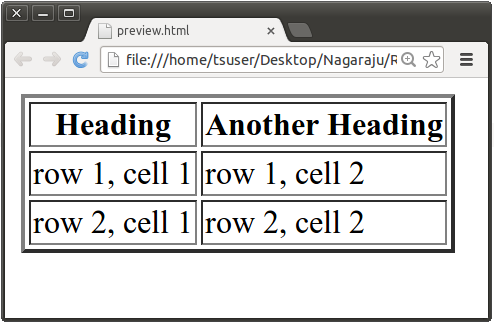
\includegraphics[scale=.25]{tables-heading.png}
\end{figure}
\end{minipage}
\end{frame}

\begin{frame}[fragile]{Tables}
\textbf{Cell Padding} specifies the space between the cell wall and the cell content in pixels.

\begin{minipage}{7cm}
\begin{lstlisting}
<table border = ``5'' cellpadding = ``10''>
    <tr>
        <td>1</td>
        <td>2</td>
    </tr>
    <tr>
        <td>3</td>
        <td>4</td>
    </tr>
</table>
\end{lstlisting}
\end{minipage}
\quad
\begin{minipage}{2cm}
\begin{figure}[H]
 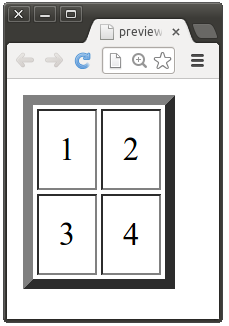
\includegraphics[scale=.3]{tables-cell-padding.png}
\end{figure}
\end{minipage}
\end{frame}

\begin{frame}[fragile]{Tables}
\textbf{Cell Spacing} Specifies the space between cells in pixels.

\begin{minipage}{7cm}
\begin{lstlisting}
<table border = ``5'' cellspacing = ``10''>
    <tr>
        <td>1</td>
        <td>2</td>
    </tr>
    <tr>
        <td>3</td>
        <td>4</td>
    </tr>
</table>
\end{lstlisting}
\end{minipage}
\quad
\begin{minipage}{2cm}
\begin{figure}[H]
 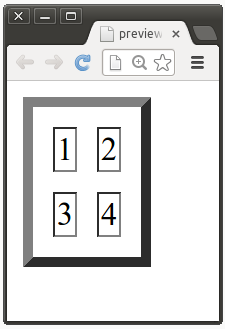
\includegraphics[scale=.3]{tables-cell-spacing.png}
\end{figure}
\end{minipage}
\end{frame}

\begin{frame}{Tables}
Table width
\begin{itemize}
 \item The width attribute can be used to define the width of a table
 \item It is defined as a fixed width in pixels irrespective of window size
 \item A relative table width is specified as a percentage of the width of the viewing window.
\end{itemize}
\begin{block}{Example}
\lstinline!<table width = ``550px''>...</table>!
    Or
\lstinline!<table width = ``80\%''>...</table>!
\end{block}
\end{frame}

\begin{frame}{Tables}
\textbf{Colspan and Rowspan}

\vspace{1pc}
Table cells can span across more than one column or row
\begin{itemize}
 \item \textbf{COLSPAN}  defines number of columns across 
 \item \textbf{ROWSPAN}  defines number of rows down
\end{itemize}
\begin{figure}[H]
 \centering
 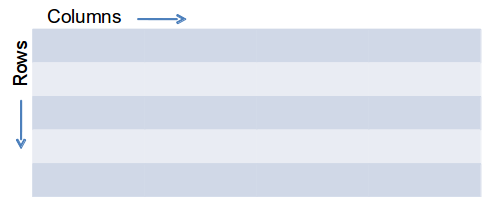
\includegraphics[scale=.3]{tables-col-row-span.png}
\end{figure}
\end{frame}

\begin{frame}[fragile]{Tables}
Colspan Example

\begin{minipage}{7cm}
\begin{lstlisting}
<table border = ``1''>
    <tr>
        <td>1</td>
        <td colspan = ``2''>2  3</td>
    </tr>
    <tr>
        <td>4</td>
        <td>5</td>
        <td>6</td>
    </tr>
    <tr>
        <td>7</td>
        <td>8</td>
        <td>9</td>
    </tr>
</table>
\end{lstlisting}
\end{minipage}
\quad
\begin{minipage}{2cm}
\begin{figure}[H]
 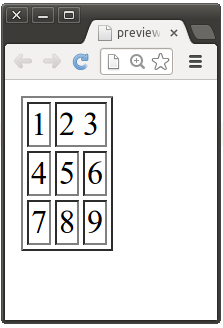
\includegraphics[scale=.3]{tables-colspan-ex.png}
\end{figure}
\end{minipage}
\end{frame}

\begin{frame}[fragile]{Tables}
Rowspan example

\begin{minipage}{7cm}
\begin{lstlisting}
<table border = ``1''>
    <tr>
        <td>1</td>
        <td rowspan = ``2''>2 5</td>
        <td>3</td>
    </tr>
    <tr>
        <td>4</td>
        <td>6</td>
    </tr>
    <tr>
        <td>7</td>
        <td>8</td>
        <td>9</td>
    </tr>
</table>
\end{lstlisting}
\end{minipage}
\quad
\begin{minipage}{2cm}
\begin{figure}[H]
 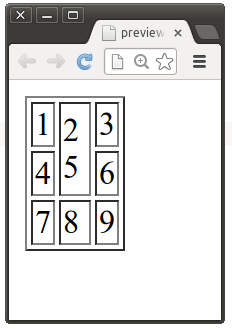
\includegraphics[scale=.3]{tables-rowspan-ex.png}
\end{figure}
\end{minipage}
\end{frame}

\begin{frame}[fragile]{Tables}
Rowspan and Colspan Example

\begin{minipage}{7cm}
\begin{lstlisting}
<table border = ``1''>
    <tr>
        <td>1</td>
        <td colspan =``2''>2</td>
    </tr>
    <tr>
        <td rowspan = ``2''>3</td>
        <td>4</td>
        <td>5</td>
    </tr>
    <tr>
        <td>6</td>
        <td>7</td>
    </tr>
</table>
\end{lstlisting}
\end{minipage}
\quad
\begin{minipage}{3cm}
\begin{figure}[H]
 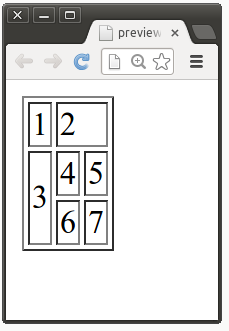
\includegraphics[scale=.4]{tables-rowspan-colspan.png}
\end{figure}
\end{minipage}
\end{frame}

\begin{frame}{HTML Basics}
 \begin{figure}[H]
 \begin{center}
   
\includegraphics[scale=.3]{qa.png}   
 \end{center}
  \end{figure}
\end{frame}

\end{document}
